\documentclass[a4paper, 12pt]{article}

\usepackage{a4,amssymb,color,graphicx}

\usepackage[ngerman]{babel}
\usepackage[T1]{fontenc}
\usepackage{ae,aecompl}
\usepackage[utf8]{inputenc}
%zum kuerzen
\usepackage{cancel}
%\usepackage{wrapfig}
\usepackage{fancyvrb}
\usepackage{amsmath}
\usepackage{amstext}
\usepackage{epstopdf}

%huebsche kopfzeilen
\usepackage{fancyhdr}
\pagestyle{fancy}
\fancyhead[C]{}
\fancyfoot[C]{}
\fancyfoot[RE]{\thepage}
\fancyfoot[LO]{\thepage}
\renewcommand{\headrulewidth}{0.4pt}
\renewcommand{\footrulewidth}{0.4pt}
\textheight=580pt


%caption centern
\usepackage{ccaption}
\captionstyle{\centerlastline}
%Unterobjekte
\usepackage{subcaption}

\newcommand{\mensch}[1]{\textsc{#1}}	% Wichtige Physiker
\newcommand{\D}{\mbox{d}}				% Fuer gerade d in dx/dy
\newcommand{\VE}{\boldsymbol} %Für fette Vektoren

%%Vor dem drucken unbedignt auskommentieren -> reine bildschirmschrift - liest sich besser ;)
%\renewcommand{\familydefault}{phv}
\begin{document}

 \begin{titlepage}
 \begin{figure*}[t]
 \includegraphics[height=2cm]{georg} \hfill
 \end{figure*}

\normalsize
\vspace{1cm}

\begin{center}
\Large Physikalisches A-Praktikum \\ \vspace{1cm}
\hrule \vspace{3mm}
\large {} \\
\Huge{\bf STED-Mikroskopie}
\vspace{5mm}
\hrule
\end{center}

\normalsize

\begin{table}[!h]
\begin{center}

  \begin{tabular}{ll}
  Praktikant: &Philip Marszal\\
   &\\
   &\\
  Betreuer: & \\
  &\\
  Gruppe: &\\
  &\\
  Durchgeführt: &\\
  Abgegeben: &\\

\vspace{1cm}& \\
  E-Mail: & \ttfamily philip.marszal@stud.uni-goettingen.de\\
\end{tabular}
\end{center}
\end{table}
\vspace{2cm}
\flushright\fbox{
\begin{minipage}{5cm}
\hfill\vspace{2cm}\\
\begin{flushright}
\footnotesize{Testat}
\end{flushright}
\end{minipage}}
\end{titlepage}

\thispagestyle{empty}
\newpage
\thispagestyle{empty}
\tableofcontents
\newpage

\pagestyle{fancy}
\setcounter{page}{1}

\section{Einleitung}

\section{Theorie}
%Einleitung mit Motivation des Versuchs, Vergleich zu anderen hochauflösenden
%Mikroskopietechniken mit Literaturrecherche (ca. 1 Seite).
\subsection{Lichtmikroskopie}
STED-Mikroskopie ist eine Form der Lichtmikroskopie, die eine besonders gute Auflösung erreicht im Vergleich zu klassischen Mikroskopen.
Das klassische Lichtmikroskop basiert auf einem simplen Aufbau aus Linsen, wie er für den einfachsten Fall in Abb. \ref{fig:lightmic} zu sehen ist.
\begin{figure}
	\centering
	\includegraphics[width=0.75\textwidth]{}
\end{figure}
Im simpelsten Fall wirft die erste Linse, das Objektiv, ein Bild in die Fokusebene der zweiten Linse, dem Okular \cite{Dem2}.
Der kleinst mögliche Abstand zweier Punkte unter dem noch zwei getrennte Punkte erkannt werden können ist die Auflösung des Mikroskops.
Sie ist bei der Lichtmikroskopie grundlegend durch Beugung beschränkt.
Beugung bewirkt, dass das Bild eines Punktes kein weiterer Punkt ist sondern eine mithilfe der Besselfunktion beschriebene Verteilung konzentrischer Ringe \cite{Born}, die sogenannte Punktspreizfunktion (PSF, \emph{point spread function}).
Insbesondere hat das Zentrum der Ringe, das erste Maximum, eine endliche Ausdehnung.
Dieses erste Maximum wird im Allgemeinen als Arrayscheibe bezeichnet.
Liegen zwei Punkte zu dicht beieinander so überlappen sich ihre Arrayscheiben, und die Punkte können nicht mehr aufgelöst werden.\\
Die minimale Distanz, die zwei Punkte voneinander haben müssen, um als zwei Punkte erkannt zu werden, wird durch Auflösungskriterien bestimmt.
Das Sparrow'sche Auflösungskriterium \cite{sparrow} besagt, dass zwei Punkte (im Original Sterne) dann noch aufgelöst werden können, wenn die Intensitätsverteilung zwischen zwei Maxima gerade noch ein Minimum aufweist.
Eine konservativere Definition eines Auflösungskriteriums ist hingegen das Rayleighkriterium, welches in diesem Versuch hauptsächlich benutzt wird.
Nach Rayleigh werden zwei Punkte genau dann noch aufgelöst, wenn das Maximum eines Punktes in das Minimum des anderen fällt \cite{Dem2}.
Dies entspricht dem Abstand des ersten Minimums der PSF vom ersten Maximum und ist gegeben durch die Formel \ref{eq:rayleigh}
\begin{align}
	d_{min} = 1.22\cdot \frac{\lambda}{2n\sin \alpha}. \label{eq:rayleigh}
\end{align}
Hierbei beschreibt $\lambda$ die Wellenlänge des zu Mikroskopieren verwendeten Lichts, $n$ den Brechungsindex des Mediums und $\alpha$ den maximalen Öffnungswinkel der Obejktivlinse.
Der Term $n\sin\alpha$ wird als die numerische Apertur eines Objektivs $NA$ bezeichnet \cite{Born}.
\\
Experimentell ist die Auflösung nach Rayleigh oder Sparrow nur schwer zu messen. 
Als Maß für die Auflösung kann jedoch die Halbwertsbreite der PSF (FWHM, \emph{full width at half maximum} benutzt werden. 
%• Erklärung Fluoreszenz und Fluoreszenzmikroskopie mit Jablonski-Diagramm.
\subsection{Fluoreszenzmikroskopie}
Eine besondere Art von Lichtmikroskopie ist die Fluoreszenzmikroskopie.
Im Gegensatz zur klassischen Mikroskopie wird nicht, das von der Probe reflektierte oder an der Probe gebrochene Licht im Okular detektiert, vielmehr wird die Probe selbst zum Leuchten angeregt.
Das Prinzip der Fluoreszenz besteht darin Moleküle mithilfe von Licht einer spezifischen Wellenlänge in einen energetisch höheren Zustand zu versetzen. 
Bei der Rückkehr der Moleküle in ihren Grundzustand senden diese Photonen aus. 
Die Wellenlänge der absorbierten und emittierten Photonen hängt von der Verteilung der Energieniveaus des Moleküls ab. Sie ist in sogenannten Jablonski-Diagrammen schematisch dargestellt (siehe Abb. \ref{fig:jablonski}).
In der Regel befindet sich ein angeregtes Molekül nicht nur in einem elektronisch angeregten Zustand sondern auch in einem angeregten Schwingungszustand.
Durch die Relaxation aus dem Schwingungszustand besitzt das Molekül eine geringere Energie vor der Emission eines Photons als unmittelbar nach der Anregung.
Dies führt dazu, dass emittiertes Licht eine größere Wellenlänge hat als absorbiertes Licht. Dieses Phanomen trägt den Namen Stokes-Shift \cite{haken}.
\\
Der Vorteil der Fluoreszenzmikroskopie gegenüber der herkömmlichen Lichtmikroskopie ist, dass gezielt Strukturen mit Fluoreszenzfarbstoff präpariert werden können (über Proteine u.ä.) und ungewollte Brechungszentren ausgeblendet werden können.
%• Konfokal-Mikroskopie: gehen Sie hier bitte kurz auf die Rolle der Lochblende ein
\subsection{Konfokalmikroskopie}
Eine Form der Fluoreszenzmikroskopie ist die Konfokalmikroskopie. 
Konfokalmikroskopie beleuchtet meist mit einem fokusierten Laser nur einen kleinen Ausschnitt der Probe. Allerdings wird die gesamte Probe abgerastert, sodass erst nach dem Zusammenfügen der einzelnen Flecken ein vollständiges Bild entsteht.
\\
Das Besondere an der Konfokalmikroskopie ist eine im Detektionsstrahlengang eingebrachte Lochblende. Ihre Funktion ist die Abschirmung von Licht, welches nicht von der Fokusebene stammt. Dadurch ist es möglich einen hohen Kontrast zu erzielen und nur einen scharfen Ausschnitt einer Ebene der Probe aufzunehmen.
\\
Die axiale Auflösung eines Konfokalmikroskops ist durch Gleichung (\ref{eq:axial}) bestimmt \cite{beyer}.
\begin{align}
	d_{axial} = \frac{0.88\cdot \lambda_{ex}}{n-\sqrt{n^2-NA^2}}. \label{eq:axial}
\end{align}
Hier bezeichnet $\lambda_{ex}$ die Wellenlänge der Fluoreszenzanregung. 
Die Dicke der beleuchteten Schicht lässt sich nach Gleichung (\ref{eq:slice}) bestimmen \cite{beyer}.
\begin{align}
	d_{schicht} = \sqrt{\left( \frac{0.88\lambda_{ex}}{n-\sqrt{n^2-NA^2}}\right)^2 + \left( \frac{\sqrt{2}\cdot n \cdot PH}{NA}\right)^2}. \label{eq:slice}
\end{align}
$PH$ bezeichnet den Durchmeser der konfokalen Lochblende.
%und nennen die zu erwartende Tiefendiskriminierung.
%• Beugungsgrenze in der Mikroskopie, Airy-Scheibe, beugungsbegrenzte PSF (rigo-
%rose Herleitung nicht nötig!), die Sie später für die Auswertung benötigen, Auflö-
%sungskriterien Rayleigh, Sparrow und axiale Auflösung.
%• STED-Mikroskopie: Erklärung des zugrundeliegenden Prinzips zur Auflösungs-
%erhöhung mit eigenen Worten (wichtig!).
\subsection{STED-Mikroskopie}
%• Motivation / Definition des Sättigungsfaktors aus den Ratengleichungen von An-
%regung und stimulierter Emission.
%• Skalierung der Auflösung mit der Intensität.
%• Die Theorie soll sich auf gepulste Systeme beziehen, der Fall mit Dauerstrichla-
%sern ist leider nicht analytisch lösbar, aber in den experimentellen Ergebnissen
%vergleichbar.

%\subsection{Molekulardynamik Simulation}
Die numerische Behandlung von Molekülen basiert zunächst auf der quantenmechanischen Beschreibung von Molekülen.
Allerdings stößt die Berechnung von quantenmechanischen Systemen bereits ab einer Zahl von 10 Atomen an ihre Grenzen.
Um dennoch sinnvolle numerische Ergebnisse in endlicher Zeit zu erhalten, werden für die Molekulardynamik Simulationen eine Reihe von Approximationen eingesetzt.
So wird die Bewegung der Elektronen eines Atoms, von der Bewegung des Kerns, entkoppelt, indem angenommen wird, dass der Atomkern sich im Vergleich zu den Elektronen sehr langsam bewegt.
Damit kann die Bewegung der Elektronen als die Bewegung in einem ruhenden Potential der Kerne betrachtet werden.
Der Einfluss der Elektronen auf den Atomkern wird wiederum durch ein durch die Elektronen verursachtes effektives Potential beschrieben.
\\ \noindent
Dieses effektive Potential wird durch die Koordinaten des Atomkerns bestimmt. Es berücksichtigt sowohl Bindungen in einem Molekül als auch langreichweitige Wechselwirkungen wie die van-der-Waals-Kräfte.
\\ \noindent
Die Bewegung der Atomkerne kann darauf hin nach den klassischen Bewegungsgleichungen integriert werden.
Hier wird der \emph{leap frog} Algorithmus zur Integration verwendet:
\begin{align}
v\left(t+\frac{\Delta t}{2}\right) = v\left(t-\frac{\Delta t}{2}\right) + \frac{F(t)}{m}\Delta t, \\
r\left(t+\frac{\Delta t}{2}\right) = r(t) + v\left(t+\frac{\Delta t}{2}\right)\Delta t.
\end{align}
\\ \noindent
Des weiteren müssen für eine sinnvolle Simulation einige technische Grenzen gesetzt werden.
Die Integrationsschrittweite wird den schnellsten erwarteten Fluktuationen entsprechend gewählt. In diesem Versuch sind dies Fluktuationen von Wasserstoffatomen, die auf einer Zeitskala von $10^{-14}$~s geschehen. Als Schrittweite wird deswegen $\Delta t = 10^{-15}$~s gewählt.
Um Randeffekte zu vermeiden werden periodische Randbedingungen gewählt, wodurch prinzipiell ein unendlich großes System simuliert wird.
\\ \noindent
Die Molekulardynamik Simulation wird in diesem Versuch mit dem Softwarepaket \emph{GROMACS} durchgeführt.

\subsection{Principal Component Analysis}
Die Hauptkomponentenanalyse oder PCA (engl. Principal Component Analysis) ist eine Methode der Datenanalyse, die aus einem Datensatz Linearkombinationen von Variablen erzeugt die maximalen Einfluss auf die Dynamik haben.
Dazu wird zunächst die Kovarianz-Matrix des Datensatzes bestimmt. Anschließend wird diese diagonalisiert und die Diagonalelemente ihrer Größe nach geordnet. Nun werden die Daten in die Basis mit diagonaler Kovarianz-Matrix transformiert.
Die Basisvektoren dieser Basis entsprechen den Hauptkomponenten oder PCs (engl. Principal Components).
Das zugehörige Diagonalelement der Kovarianz-Matrix entspricht der auf dieser Achse auftretender Varianz der Daten.
\\ \noindent
Die Hauptkomponenten mit der größten Varianz entsprechen den Variablen mit der stärksten Aussagekraft über den Zustand des Systems. Vernachlässigt man Hauptkomponenten geringer Varianz, so lässt sich die Dimensionalität des Datensatzes stark verringern ohne Information einzubüßen.
In diesem Versuch wird es hilfreich sein komplexe Proteinbewegungen auf zwei essentielle Bewegungen zu reduzieren um die Arbeitsweise des Proteins zu untersuchen.

\section{Durchführung}
\section{Durchführung}
Das Phänomen der Rayleigh-Benard-Konvektion wird sowohl numerisch als auch experimentell untersucht.
\subsection{Simulation}
Mithilfe des Programms \emph{Comsol Multiphysics} wird die Rayleigh-Benard-Konvektion in einer zweidimensionalen Box simuliert. 
Die Simulation wird für die Rayleigh-Zahlen $10^3, 10^4, 10^5$ und $10^6$ durchgeführt. 
Ausgegeben werden dabei die Temperatur- und Geschwindigkeitsprofile entlang der Achse durch die Mitte der Box.
\\
Zudem wird die Nusselt-Zahl als das Integral des Wärmegradienten über die Grenzfläche der Box bestimmt.

\subsection{Experimentelle Betrachtung}
\subsubsection{Schattenwurfmethode}
Zunächst wird die Dynamik des Fluids im Versuchsaufbau, visuell beschrieben.
Dazu wird die Glasbox so beleuchtet, dass auf einer Seite durch die Plumes erzeugte Schatten zu erkennen sind.
Die Schatten entstehen durch die Brechung des Lichts an starken Dichtegradienten des Fluids, die Folge von Temperaturunterschieden sind.
\\
Die Geschwindigkeit der Plumes wird mithilfe einer Stoppuhr gemessen. 
Es werden sowohl auf einer Seite aufsteigende warme Plumes, als auch auf der anderen Seite fallende kalte Plumes gemessen.
\\
Die Strecke über die gemessen wird beträgt ca. 2.5~cm. Für jede Seite werden 10 Messwerte gesammelt.
\subsubsection{Beweglicher Thermistor}
Das Temperatur- und Geschwindigkeitsprofil des Fluids wird nun mit einem einzelnen Thermistor bestimmt.
Der Thermistor wird zunächst direkt an der warmen Platte in der Mitte der Box positioniert. 
Mit einem bereitgestellten Messprogramm werden nun 2048 Messwerte der Temperatur mit einer Abtastfrequenz von 9.5~Hz auf genommen. 
\\ 
Dann wird der Thermistor um 1~cm nach oben verschoben, und eine Messung für die neue Höhe gestartet. Dies wird bis zu einer Höhe von 10~cm durchgeführt.
\\
Für die ersten 1.5~cm werden die Messungen alle 0.1~cm durchgeführt. 
Für die Bestimmung der thermischen Grenzschicht wird zudem eine noch höhere Auflösung benötigt, weswegen zusätzliche Messwerte bei 0.05, 0.15, 0.25 und 0.35~cm aufgenommen werden, die allerdings nur aus 512 Messpunkten bestehen.

\subsubsection{Thermistorarray}
Anschließend wird eine lange Messung mit einem Thermistorarray aus sechs Thermistoren durchgeführt.
Mit allen Thermistoren wird über 30~Stunden hinweg die Temperatur gemessen.
Aus der zeitlichen Korrelation der Messwerte der einzelnen Thermistoren lässt sich die Geschwindigkeit von Plumes bestimmen.


%\section{Auswertung}
\section{Auswertung}
\subsection{Schattenspiel}
Die Temperaturen der Heiz- und Kühlplatte wurden zu \SI{11.05}{\celsius} und \SI{19.84}{\celsius} bestimmt. Daraus und aus den Abmessungen der Zelle wird die Rayleighzahl nach \cref{eq:rayleigh} zu ca. $\text{Ra} = 1.01\cdot 10^{9}$ bestimmt.
\\
Die Messung der Geschwindigkeiten der Plume-Schatten ergibt für aufsteigende Plumes \SI{0.50\pm0.01}{\centi\meter\per\second}, und für fallende Plumes ergibt sich eine mittlere Geschwindigkeit von \SI{0.71\pm0.02}{\centi\meter\per\second}.
Für die Berechnung der Reynoldszahl wird nur die Messung für die aufsteigenden Plumes herangezogen, da es bei der Messung der fallenden Plumes zu einem systematischen Fehler durch die Fokusebene der Beleuchtung kommt. Es ergibt sich eine Reynoldszahl von $\text{Re}=10^{3}$.
\\ % Aufgabe 15 

\subsection{Vorbereitung: Thermistor}
Da Geschwindigkeit der Plumes über eine Fouriertransformation der gemessenen Temperatur bestimmt wird, können Fehler in der Messung durch den Einfluss von Störfrequenzen auf die Thermistoren auftreten.
Um mögliche Störfrequenzen zu identifizieren, wird zunächst eine Messung mit einer Abtastfrequenz von \SI{250}{\hertz} durchgeführt. 
Diese kann Störfrequenzen von 0 bis \SI{250}{\hertz} aufdecken.
\\
Eine starke, wenn auch zu erwartende, Störung tritt bei \SI{50}{\hertz} auf, und wird durch das Stromnetz verursacht (siehe \cref{fig:stoer}).
Durch \cref{eq:frequency} kann nun eine Abtastfrequenz gewählt werden, die das Auftreten der Störfrequenz in der Messung so verschiebt, dass die Messergebnisse unbeeinflusst bleiben. Deswegen wurde die Abtastfrequenz als \SI{11.5}{\hertz} gewählt.
\begin{align}
	|f_{\text{real}}- f_{\text{measured}} | = \lfloor\frac{f_{\text{real}}}{f_{\text{max}}}\rfloor \cdot f_{\text{max}}. \label{eq:frequency}
\end{align}
\begin{figure}
	\input{Figures/power_250}\caption{Ergebnis der Suche nach Störfrequenzen mit einer Abtastrate von \SI{250}{\hertz}. Die einzige erkennbare Störfrequenz liegt bei \SI{50}{\hertz} und wird durch das Stromnetz verursacht.}\label{fig:stoer}
\end{figure}
\\

\subsection{Temperaturmessungen}
Aus den Messungen der Temperatur als Funktion des Abstandes ergibt sich das in \cref{fig:temp-prof} dargestellte Temperaturprofil. Es ist sowohl das Ergebnis der Messung mit dem beweglichen Thermistor, als auch die Messung der Temperatur mit dem Thermistor-Array zu sehen. 
\cref{fig:temp-array} hingegen zeigt allein die Messung mit dem Thermistorarry.
\\
\begin{figure}
\centering
\includegraphics[width=\textwidth]{plots/T_profile2.pdf}
\caption{Temperaturprofil der unteren Hälfte der Zelle, als Funktion des Abstandes von der Heizplatte. Zu sehen ist die vollständige Messreihe mittels beweglichem Thermistor, und die ersten drei Messwerte des Thermistorarrays.
Zur Bestimmung der thermischen Grenzschicht wurde der Schnittpunkt zweier linearer Fits bestimmt.}\label{fig:temp-prof}
\end{figure}
Aus dem Temperaturprofil lässt sich die Nusseltzahl, über die thermische Grenzschicht bestimmen. Der bestimmte Schnittpunkt der beiden in \cref{fig:temp-prof} zu sehenden Fits liegt bei einem Abstand von \SI{0.25\pm0.4}{\centi\meter}. Nach \cref{eq:nusselt} ergibt sich dies zu einer Nusseltzahl von $\text{Nu}=\SI{40\pm7}{}$.
\\
\begin{figure}
	\centering
	\includegraphics[width=\textwidth]{plots/T_korr_profile.pdf}
	\caption{Messungen des Temperaturprofils mithilfe des Thermistorarrays. Zu sehen sind die Mittelwerte der 30-stündigen Messung, für jeden Thermistor bzw. seine Position.}\label{fig:temp-array}
\end{figure}
Die in \cref{fig:temp-prof, fig:temp-array} dargestellten Profile lassen sich mit den aus der Simulation gewonnenen Profilen für unterschiedliche Rayleighzahlen vergleichen.
Diese sind in \cref{fig:sim-temp} dargestellt.
\\
\begin{figure}
	\centering
	\includegraphics[width=\textwidth]{plots/T_sim_Profile.pdf}
	\caption{Temperaturprofile einer Rayleigh-Benard-Zelle zu verschiedenen Rayleighzahlen. Unterlegt ist die mittels der Methode aus \cref{sec:grenz} ermittelte Grenzschicht. Für die Simulation bei $\text{Ra}=10^3$ lässt sich kein sinnvoller Wert für die Grenzschicht angeben, da das gesamte Temperaturprofil linear verläuft, d.h. der gesamte Wärmetransport diffusiv erfolgt. Dies entspricht der Theorie nach einer Nusseltzahl von 1.}\label{fig:sim-temp}
\end{figure}
Für die 30-stündige Messung ist es interessant die Verteilung der Messwerte zu betrachten. \cref{fig:hist} zeigt Histogramme der gemessenen Werte über die gesamte Messreihe hinweg. Man erkennt, dass das Maximum der Verteilungen für jeden Thermistor in etwa bei der gleichen Temperatur \SI{15.5}{\celsius} liegt. 
Allerdings kommt es durch die Nähe zur Heiz- bzw. Kühlplatte zu häufigen Messung von Temperaturen mit einer starken Abweichung vom Maximum.
Der Thermistor in der Nähe der Heizplatte misst häufiger Temperaturen über der Durchschnittstemperatur, während beim Thermistor an der Kühlplatte häufiger niederigere Temperaturen gemessen werden.
Dieser Effekt lässt sich abgeschwächt auch in den weiter entfernten Thermistoren erkennen.
\begin{figure}
	\centering
	\includegraphics[width=\textwidth]{plots/T_hist.pdf}\caption{Verteilung der Messwerte der einzelnen Thermistoren als Funktion der Temperatur. Der Abstand bezeichnet den Abstand von der Heizplatte. Die Histogramme sind auf einer logarithmischen Skala aufgetragen. Bei den Lücken in den Histogrammen, handelt es sich um Fehler, die Messwerte aus diesen Boxen auf die benachbarten Boxen verteilen.}\label{fig:hist}
\end{figure}

\subsection{Geschwindigkeitsprofile}
Über die Messung der Temperatur mit dem beweglichen Thermistor lässt sich das Geschwindigkeitsprofil der Zelle ermitteln.
Dazu wird ausgenutzt, dass entstehende Plumes in etwa dem Verlauf der Konvektionswalze folgen, und in erster Näherung die gleiche Geschwindigkeit besitzen.
\\
In der mit dem Thermistor an einer Höhe aufgenommenen Zeitreihe sind Plumes als ein vorübergehender Anstieg bzw. Abfall der Temperatur zu erkennen. 
Die Geschwindigkeit des Plumes ist invers proportional zur Breite der Senke bzw. des Hügels.
Diese ist wiederum charakterisiert, durch die Frequenzzusammensetzung des Plumes im Fourierraum.
In \cref{fig:abbruch} ist eindeutig die größte Frequenz des Plume-Bündels zu erkennen. Diese Abbruchfrequenz ist direkt proportional zur durchschnittlichen Geschwindigkeit der Plumes in diesem Abstand von der Heizplatte.
\\
Das Geschwindigkeitsprofil der unteren \SI{10}{\centi\meter} ist in in \cref{fig:vprof_freq} zu sehen. 
Das Profil der Abbruchfrequenzen $f_c$ entspricht hier dem Verlauf des Geschwindigkeitsprofils.
Der lineare Fit der ersten Werte zeigt, dass selbst an der Heizplatte eine Geschwindigkeit messbar ist.
\\
\begin{figure}
	\input{Figures/power_0000}\caption{Ermittlung der Abbruchfrequenz einer Messung. Dieses Beispiel zeigt die Bestimmung der Abbruchfrequenz für die Messung der Temperatur in unmittelbarer Nähe der Platte. }\label{fig:abbruch}
\end{figure}
\begin{figure}
	% GNUPLOT: LaTeX picture with Postscript
\begingroup
  \makeatletter
  \providecommand\color[2][]{%
    \GenericError{(gnuplot) \space\space\space\@spaces}{%
      Package color not loaded in conjunction with
      terminal option `colourtext'%
    }{See the gnuplot documentation for explanation.%
    }{Either use 'blacktext' in gnuplot or load the package
      color.sty in LaTeX.}%
    \renewcommand\color[2][]{}%
  }%
  \providecommand\includegraphics[2][]{%
    \GenericError{(gnuplot) \space\space\space\@spaces}{%
      Package graphicx or graphics not loaded%
    }{See the gnuplot documentation for explanation.%
    }{The gnuplot epslatex terminal needs graphicx.sty or graphics.sty.}%
    \renewcommand\includegraphics[2][]{}%
  }%
  \providecommand\rotatebox[2]{#2}%
  \@ifundefined{ifGPcolor}{%
    \newif\ifGPcolor
    \GPcolortrue
  }{}%
  \@ifundefined{ifGPblacktext}{%
    \newif\ifGPblacktext
    \GPblacktexttrue
  }{}%
  % define a \g@addto@macro without @ in the name:
  \let\gplgaddtomacro\g@addto@macro
  % define empty templates for all commands taking text:
  \gdef\gplbacktext{}%
  \gdef\gplfronttext{}%
  \makeatother
  \ifGPblacktext
    % no textcolor at all
    \def\colorrgb#1{}%
    \def\colorgray#1{}%
  \else
    % gray or color?
    \ifGPcolor
      \def\colorrgb#1{\color[rgb]{#1}}%
      \def\colorgray#1{\color[gray]{#1}}%
      \expandafter\def\csname LTw\endcsname{\color{white}}%
      \expandafter\def\csname LTb\endcsname{\color{black}}%
      \expandafter\def\csname LTa\endcsname{\color{black}}%
      \expandafter\def\csname LT0\endcsname{\color[rgb]{1,0,0}}%
      \expandafter\def\csname LT1\endcsname{\color[rgb]{0,1,0}}%
      \expandafter\def\csname LT2\endcsname{\color[rgb]{0,0,1}}%
      \expandafter\def\csname LT3\endcsname{\color[rgb]{1,0,1}}%
      \expandafter\def\csname LT4\endcsname{\color[rgb]{0,1,1}}%
      \expandafter\def\csname LT5\endcsname{\color[rgb]{1,1,0}}%
      \expandafter\def\csname LT6\endcsname{\color[rgb]{0,0,0}}%
      \expandafter\def\csname LT7\endcsname{\color[rgb]{1,0.3,0}}%
      \expandafter\def\csname LT8\endcsname{\color[rgb]{0.5,0.5,0.5}}%
    \else
      % gray
      \def\colorrgb#1{\color{black}}%
      \def\colorgray#1{\color[gray]{#1}}%
      \expandafter\def\csname LTw\endcsname{\color{white}}%
      \expandafter\def\csname LTb\endcsname{\color{black}}%
      \expandafter\def\csname LTa\endcsname{\color{black}}%
      \expandafter\def\csname LT0\endcsname{\color{black}}%
      \expandafter\def\csname LT1\endcsname{\color{black}}%
      \expandafter\def\csname LT2\endcsname{\color{black}}%
      \expandafter\def\csname LT3\endcsname{\color{black}}%
      \expandafter\def\csname LT4\endcsname{\color{black}}%
      \expandafter\def\csname LT5\endcsname{\color{black}}%
      \expandafter\def\csname LT6\endcsname{\color{black}}%
      \expandafter\def\csname LT7\endcsname{\color{black}}%
      \expandafter\def\csname LT8\endcsname{\color{black}}%
    \fi
  \fi
  \setlength{\unitlength}{0.0500bp}%
  \begin{picture}(7936.00,4534.00)%
    \gplgaddtomacro\gplbacktext{%
      \csname LTb\endcsname%
      \put(946,704){\makebox(0,0)[r]{\strut{} 0}}%
      \put(946,1417){\makebox(0,0)[r]{\strut{} 0.2}}%
      \put(946,2130){\makebox(0,0)[r]{\strut{} 0.4}}%
      \put(946,2843){\makebox(0,0)[r]{\strut{} 0.6}}%
      \put(946,3556){\makebox(0,0)[r]{\strut{} 0.8}}%
      \put(946,4269){\makebox(0,0)[r]{\strut{} 1}}%
      \put(1336,484){\makebox(0,0){\strut{} 0}}%
      \put(2887,484){\makebox(0,0){\strut{} 3}}%
      \put(4438,484){\makebox(0,0){\strut{} 6}}%
      \put(5988,484){\makebox(0,0){\strut{} 9}}%
      \put(7539,484){\makebox(0,0){\strut{} 12}}%
      \put(176,2486){\rotatebox{-270}{\makebox(0,0){\strut{}$f_c~[\si{\hertz}]$}}}%
      \put(4308,154){\makebox(0,0){\strut{}Abstand von der Heizplatte~[\si{\centi\meter}]}}%
    }%
    \gplgaddtomacro\gplfronttext{%
    }%
    \gplgaddtomacro\gplbacktext{%
      \csname LTb\endcsname%
      \put(4297,2740){\makebox(0,0)[r]{\strut{} 0.5}}%
      \put(4297,4042){\makebox(0,0)[r]{\strut{} 1}}%
      \put(4667,2260){\makebox(0,0){\strut{} 0}}%
      \put(5857,2260){\makebox(0,0){\strut{} 0.5}}%
      \put(7047,2260){\makebox(0,0){\strut{} 1}}%
    }%
    \gplgaddtomacro\gplfronttext{%
    }%
    \gplbacktext
    \put(0,0){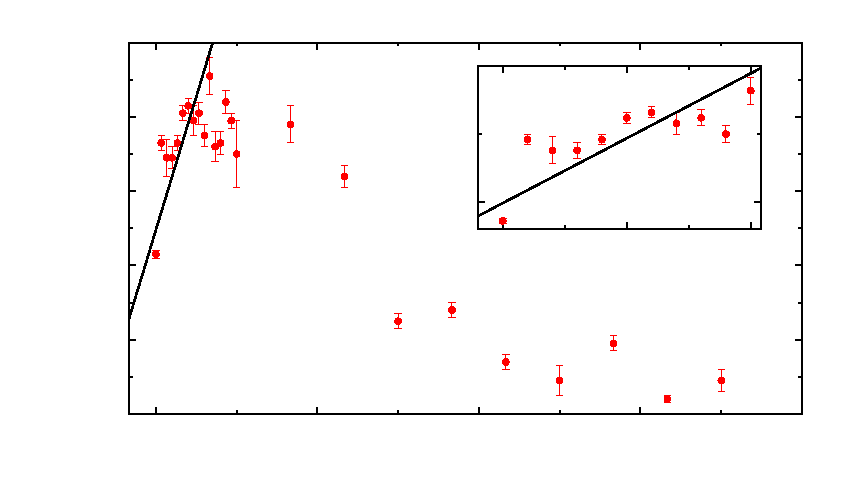
\includegraphics{v_prof_fc}}%
    \gplfronttext
  \end{picture}%
\endgroup
\caption{Zu sehen ist die Abhängigkeit der Abbruchfrequenz $f_c$ in Abhängigkeit von dem Abstand von der Heizplatte. Dieser Verlauf entspricht auch dem Geschwindigkeitsprofil in der Zelle, da die Geschwindigkeit proportional zur Abbruchfrequenz ist.}\label{fig:vprof_freq}
\end{figure}
Aus der 30-stündigen Messung lässt sich die Geschwindigkeit an fünf Stellen der Zelle bestimmen. Dazu wird aus den Temperaturmesswerten die Korrelation jeweils zweier Thermistoren gebildet.
Die Zeit $\tau$ des Maximums einer Korrelation entspricht der mittleren Zeit, die ein Plume braucht um von einem Thermistor zum anderen zu fließen.
Mit dieser Zeit und dem Abstand zwischen der betrachteten Thermistoren lässt sich die Geschwindigkeit zwischen diesen bestimmen.
In \cref{fig:korr} sind die Korrelationen zwischen jeweils benachbarten Thermistoren zu sehen. Aus den Maxima der Korrelationen ergeben sich die mittleren Geschwindigkeiten in \cref{fig:v_korr}.
Das Geschwindigkeitsprofil aus den Korrelationsmessungen spiegelt kein erwartetes Profil mit eindeutigem Minimum im Zentrum der Zelle wieder.
\\
\begin{figure}
	% GNUPLOT: LaTeX picture with Postscript
\begingroup
  \makeatletter
  \providecommand\color[2][]{%
    \GenericError{(gnuplot) \space\space\space\@spaces}{%
      Package color not loaded in conjunction with
      terminal option `colourtext'%
    }{See the gnuplot documentation for explanation.%
    }{Either use 'blacktext' in gnuplot or load the package
      color.sty in LaTeX.}%
    \renewcommand\color[2][]{}%
  }%
  \providecommand\includegraphics[2][]{%
    \GenericError{(gnuplot) \space\space\space\@spaces}{%
      Package graphicx or graphics not loaded%
    }{See the gnuplot documentation for explanation.%
    }{The gnuplot epslatex terminal needs graphicx.sty or graphics.sty.}%
    \renewcommand\includegraphics[2][]{}%
  }%
  \providecommand\rotatebox[2]{#2}%
  \@ifundefined{ifGPcolor}{%
    \newif\ifGPcolor
    \GPcolortrue
  }{}%
  \@ifundefined{ifGPblacktext}{%
    \newif\ifGPblacktext
    \GPblacktexttrue
  }{}%
  % define a \g@addto@macro without @ in the name:
  \let\gplgaddtomacro\g@addto@macro
  % define empty templates for all commands taking text:
  \gdef\gplbacktext{}%
  \gdef\gplfronttext{}%
  \makeatother
  \ifGPblacktext
    % no textcolor at all
    \def\colorrgb#1{}%
    \def\colorgray#1{}%
  \else
    % gray or color?
    \ifGPcolor
      \def\colorrgb#1{\color[rgb]{#1}}%
      \def\colorgray#1{\color[gray]{#1}}%
      \expandafter\def\csname LTw\endcsname{\color{white}}%
      \expandafter\def\csname LTb\endcsname{\color{black}}%
      \expandafter\def\csname LTa\endcsname{\color{black}}%
      \expandafter\def\csname LT0\endcsname{\color[rgb]{1,0,0}}%
      \expandafter\def\csname LT1\endcsname{\color[rgb]{0,1,0}}%
      \expandafter\def\csname LT2\endcsname{\color[rgb]{0,0,1}}%
      \expandafter\def\csname LT3\endcsname{\color[rgb]{1,0,1}}%
      \expandafter\def\csname LT4\endcsname{\color[rgb]{0,1,1}}%
      \expandafter\def\csname LT5\endcsname{\color[rgb]{1,1,0}}%
      \expandafter\def\csname LT6\endcsname{\color[rgb]{0,0,0}}%
      \expandafter\def\csname LT7\endcsname{\color[rgb]{1,0.3,0}}%
      \expandafter\def\csname LT8\endcsname{\color[rgb]{0.5,0.5,0.5}}%
    \else
      % gray
      \def\colorrgb#1{\color{black}}%
      \def\colorgray#1{\color[gray]{#1}}%
      \expandafter\def\csname LTw\endcsname{\color{white}}%
      \expandafter\def\csname LTb\endcsname{\color{black}}%
      \expandafter\def\csname LTa\endcsname{\color{black}}%
      \expandafter\def\csname LT0\endcsname{\color{black}}%
      \expandafter\def\csname LT1\endcsname{\color{black}}%
      \expandafter\def\csname LT2\endcsname{\color{black}}%
      \expandafter\def\csname LT3\endcsname{\color{black}}%
      \expandafter\def\csname LT4\endcsname{\color{black}}%
      \expandafter\def\csname LT5\endcsname{\color{black}}%
      \expandafter\def\csname LT6\endcsname{\color{black}}%
      \expandafter\def\csname LT7\endcsname{\color{black}}%
      \expandafter\def\csname LT8\endcsname{\color{black}}%
    \fi
  \fi
  \setlength{\unitlength}{0.0500bp}%
  \begin{picture}(7936.00,4534.00)%
    \gplgaddtomacro\gplbacktext{%
      \csname LTb\endcsname%
      \put(1210,704){\makebox(0,0)[r]{\strut{} 0}}%
      \put(1210,1298){\makebox(0,0)[r]{\strut{} 0.002}}%
      \put(1210,1892){\makebox(0,0)[r]{\strut{} 0.004}}%
      \put(1210,2487){\makebox(0,0)[r]{\strut{} 0.006}}%
      \put(1210,3081){\makebox(0,0)[r]{\strut{} 0.008}}%
      \put(1210,3675){\makebox(0,0)[r]{\strut{} 0.01}}%
      \put(1210,4269){\makebox(0,0)[r]{\strut{} 0.012}}%
      \put(1342,484){\makebox(0,0){\strut{} 0}}%
      \put(2891,484){\makebox(0,0){\strut{} 10}}%
      \put(4441,484){\makebox(0,0){\strut{} 20}}%
      \put(5990,484){\makebox(0,0){\strut{} 30}}%
      \put(7539,484){\makebox(0,0){\strut{} 40}}%
      \put(176,2486){\rotatebox{-270}{\makebox(0,0){\strut{}$\left(\Ta_i \star \Ta_j\right)\left(\tau\right)$~[\si{\second\squared}]}}}%
      \put(4440,154){\makebox(0,0){\strut{}$\tau$~[\si{\second}]}}%
    }%
    \gplgaddtomacro\gplfronttext{%
      \csname LTb\endcsname%
      \put(6552,4096){\makebox(0,0)[r]{\strut{}$\Ta _1 \star \Ta_2$}}%
      \csname LTb\endcsname%
      \put(6552,3876){\makebox(0,0)[r]{\strut{}$\Ta _2 \star \Ta_3$}}%
      \csname LTb\endcsname%
      \put(6552,3656){\makebox(0,0)[r]{\strut{}$\Ta _3 \star \Ta_4$}}%
      \csname LTb\endcsname%
      \put(6552,3436){\makebox(0,0)[r]{\strut{}$\Ta _4 \star \Ta_5$}}%
      \csname LTb\endcsname%
      \put(6552,3216){\makebox(0,0)[r]{\strut{}$\Ta _5 \star \Ta_6$}}%
      \csname LTb\endcsname%
      \put(6552,2996){\makebox(0,0)[r]{\strut{}Maximum}}%
    }%
    \gplbacktext
    \put(0,0){\includegraphics{v_correlation_12}}%
    \gplfronttext
  \end{picture}%
\endgroup
\caption{Korrelation benachbarter Thermistoren. Die Zeit der Maximums entspricht der Zeit, die ein Plume im Mittel braucht um die Strecke zwischen den Thermistoren zu überwinden. Zwischen dritten und viertem Thermistor liegt das Maximum bei einer größeren Zeit als erwartet, da der Abstand des dritten und vierten Thermistors größer ist.}\label{fig:korr}
\end{figure}
\begin{figure}
	\input{Figures/vel_corr_therm}\caption{Aus den Korrelationen bestimmte Werte für die Geschwindigkeit in Abhängigkeit vom Abstand von der Kühlplatte. Das erwartete Profil mit Minimum in der Mitte, wie in \cref{fig:vprof_sim} ist nicht zu erkennen.}\label{fig:v_korr}
\end{figure}
In der Simulation lässt sich das Geschwindigkeitsprofil direkt bestimmen, ohne Plumes zur Bestimmung heranziehen zu müssen.
Die gemessenen Profile sind in \cref{fig:vprof_Ra_1e3,fig:vprof_Ra_1e4,fig:vprof_Ra_1e5,fig:vprof_Ra_1e6,fig:vprof_Ra_1e7} zu sehen. 
Eine Ausbildung zweier Maxima ist ab einer Rayleighzahl von $10^4$ deutlich zu erkennen. 
Bei einer Rayleighzahl von $10^3$ jedoch ist die Geschwindigkeit $\approx 0$. 
In \cref{fig:vprof_Ra_1e3} sind demnach nur durch Diffusion verursachte Schwankungen zu sehen.
\\
\cref{fig:SimSnapshot} zeigt eine farbkodierte Momentaufnahme des Geschwindigkeits- und Temperaturfeldes. 
\\
\begin{figure}[!h]
        \centering
        \begin{subfigure}{0.5\textwidth}
        \input{./Figures/v_prof_Ra_1e3.tex}
        \caption{$\Ra = \num{e3}$}
        \label{fig:vprof_Ra_1e3}
\end{subfigure}\hfill
        \begin{subfigure}{0.5\textwidth}
        \input{./Figures/v_prof_Ra_1e4.tex}
        \caption{$\Ra = \num{e4}$}
        \label{fig:vprof_Ra_1e4}
\end{subfigure} \\
        \begin{subfigure}{0.5\textwidth}
        \input{./Figures/v_prof_Ra_1e5.tex}
        \caption{$\Ra = \num{e5}$}
        \label{fig:vprof_Ra_1e5}
\end{subfigure}\hfill
        \begin{subfigure}{0.5\textwidth}
        \input{./Figures/v_prof_Ra_1e6.tex}
        \caption{$\Ra = \num{e6}$}
        \label{fig:vprof_Ra_1e6}
\end{subfigure} \\
        \begin{subfigure}{0.5\textwidth}
        \input{./Figures/v_prof_Ra_1e7.tex}
        \caption{$\Ra = \num{e7}$}
        \label{fig:vprof_Ra_1e7}
\end{subfigure}\hfill
        \begin{subfigure}{0.5\textwidth}
                \includegraphics[width=1\textwidth]{Ra_1e7_turbolent.png}
                \caption{Snapshot für $\Ra = \num{e7}$}
                \label{fig:SimSnapshot}
         \end{subfigure}
        \caption{Ergebnisse der numerischen Bestimmung der Geschwindigkeitsprofile für die Rayleighzahlen von $10^{3}$ bis $10^7$. Zu sehen ist das zeitliche Mittel über die Achse durch das Zentrum der Box, wie sie in~(\subref{fig:SimSnapshot}) hervorgehoben ist.
Es wird nur jeder vierte Messwert durch einen Punkt dargestellt. 
        }\label{fig:SimVprof}
\end{figure}

\subsection{Bestimmung der Nusseltzahl}
Die Nusseltzahl der Simulationen wurde auf zwei unterschiedliche Arten bestimmt. 
Mithilfe von \emph{Comsol Multiphysics} wurde das Integral des Wärmegradienten über die obere Kante der Simulationsbox bestimmt.
Da der Wärmefluss in diesem Aufbau der Kontinuitätsgleichung unterliegt, kann die Linie über die integriert wird frei gewählt werden. 
Es bietet sich an eine Linie zu wählen, welche in der thermischen Grenzschicht liegt, da der Temperaturgradient dort nahezu konstant ist (siehe \cref{fig:temp-prof}).
Die Ergebnisse für jede Rayleighzahl lassen sich \cref{fig:nusselt} entnehmen. 
\\
Die zweite Methode mit der die Nusseltzahl bestimmt wurde benutzt \cref{eq:nussbound} und die dafür nötige Bestimmung der Grenzschicht. 
Eine Methode der Grenzschichtbestimmung ist der Fit zweier linearer Funktionen an das Temperaturprofil. Da in der thermischen Grenzschicht nur diffusiver Wärmetransport stattfindet, kann das Temperaturprofil durch eine Gerade beschrieben werden.
Das Ende der Grenzschicht wird durch den Schnittpunkt mit einer Gerade durch die konstante Temperatur im Zentrum der Zelle markiert. 
Für unseren wurde das Temperaturprofil außerhalb der Grenzschicht nicht mit einer Konstanten, sondern ebenfalls mit einer linearen Funktion angenähert.
\\
Diese Methode wurde sowohl auf die simulierten Messwerte angewandt, als auch auf die experimentell ermittelten. Die Ergebnisse sind ebenfalls in \cref{fig:nusselt} aufgetragen.
\\
Es ist ersichtlich, dass die Nusseltzahl über ein Potenzgesetz mit der Rayleighzahl verknüpft ist. Der Fit einer Geraden durch den doppelt-logarithmischen Plot in \cref{fig:nusselt} liefert ein Potenzgesetz der Form $\text{Nu} \propto \text{Ra}^{0.260(8)}$.
Für den Fit wurde die Gesamtheit der Messwerte verwendet.
\begin{figure}
	\centering
	\includegraphics[width=\textwidth]{plots/nusselt_fit.pdf}\caption{Nusseltzahl aufgetragen gegen die Rayleighzahl.
Der Fit ergibt ein Potenzgesetz für die Beziehung zwischen Nusseltzahl und Rayleighzahl: \mbox{$\text{Nu} \propto \text{Ra}^{0.260(8)}$}. Die Fehler der Messwerte ergeben sich aus der Standardabweichung der jeweilingen linearen Fits und verschwinden für den Großteil der der Messwerte in der logarithmischen Darstellung. Die Werte der Grenzschichtmessung unterliegen zudem einem unbestimmten systematischen Fehler, durch die Wahl der Messwerte für den Fit der linearen Funktionen.}
\label{fig:nusselt}
\end{figure}
%%%%%%%%%%%%%%%%%%%%%%%%%%%%%%%%%%
% critical rayleigh number 1707
% wikipedia rayleigh benard

%%%%%%%%%%%%%%%%%%%%%%%%%%%%%%%%%%


%	 RAYLEIGH ZAHL DES EXPERIMENTS

% ICH	 SCHATTENPROJEKTION GESCHWINDIGKEIT 

%	 STÖRFREQUENZEN
%		FORMEL

% ICH	 TEMPERATUR ALS ABSTAND DER PLATTE

% ICH	 TEMPERATUR PROFILE

% ICH	 TEMPERATUR DURCH LANGE MESSUNG

%	 GESCHWINDIGKEITSPROFIL DURCH ABBRUCHFREQUENZ

% NUR ICH:
%	GESCHWI VERGlEICH FALL, REIBUNG
%	HISTOGRAMME TEMPERATUR


%\section{Diskussion}
%\subsection{Simulation von Argon}
Betrachtet man den Verlauf der potentiellen Energie des Argon so stellt man für jede der Simulationen einen abrupten Abfall fest.
Dies ist durch den Phasenübergang gasförmig-flüssig zu erklären.
Die potentielle Energie des Gases ist durch die Summe der einzelnen effektiven Potentiale bestimmt.
Beim Kondensieren, verringern sich die Abstände zwischen den Atomen stark. Die einzelnen Argonteilchen sitzen nahezu im Minimum des Potentials fest.
Deswegen ist es möglich gewesen den Siedepunkt des Argons mithilfe der potentiellen Energie zu bestimmen.
\\ \noindent
Die in Tab. \ref{tab:siedepunkt} ermittelten Siedepunkte weichen stark von dem Literaturwert von 98~K \cite{phasediagram} ab. Auch zueinander sind die ermittelten Werte stark unterschiedlich.
Da der einzige Unterschied zwischen den Simulationen der Zeitraum der Abkühlung ist, liegt es nahe, dass dieser die entscheidende Rolle für den Siedepunkt spielt.
\\ \noindent
Besonders deutlich ist die Abweichung der 1~ns Simulation. Auffällig ist, dass das Minimum der potentiellen Energie über diesen Zeitraum nicht erreicht wird.
Sogar der mittels dem Fit ermittelte Siedepunkt wird nicht erreicht.
Hier wird deutlich, dass der Algorithmus zur Temperatursenkung nicht für sehr kleine Zeitskalen anwendbar ist.
Unter Umständen jedoch kann das Ergebnis für kleine Zeitskalen verbessert werden, wenn kleinere Integrationsschritte verwendet werden, um den Einfluss der Temperatursenkung auf das Resultat der Integration zu minimieren.
\\ \noindent
Ein gravierender Unterschied ist zwischen dem Erhitzen und Abkühlen festzustellen. In Abb. \ref{fig:cool_pot10ns}) ist zu erkennen, dass die Kurve der potentiellen Energie beim Erhitzen des flüssigen Argons ungenauer ist und keiner logistischen oder ähnlichen Kurve entspricht.
Die Bestimmung des Siedepunktes für diese Kurve war leider nicht mit einem Fit an eine Logistische Kurve möglich, weswegen nur eine Schätzung möglich ist.
Der Punkt der Maximalen Steigung ist bei ca. 8300~ps zu erkennen was einer Temperatur von ca. 105~K entspricht.
Obwohl dieser Wert näher an dem Literaturwert liegt als die zuvor bestimmten Werte, ist dennoch anzunehmen, dass aufgrund der Kurvenform das Ergebnis wesentlich ungenauer ist.
\\ \noindent
Der Schmelzpunkt von Argon kann erneut durch den rapiden Abfall der potentiellen Energie in Abb. \ref{fig:liqpot}) bestimmt werden und liegt bei ca. 50~K.
Der Literaturwert für den Schmelzpunkt von Argon bei 1~bar liegt bei 83.9~K \cite{chemicalcrc}. Da Argon keine Anomalie besitzt, wie z.B. Wasser, ist für einen höheren Druck von 5.8~bar auch ein höherer Schmelzpunkt zu erwarten.
Das Ergebnis widerspricht also den theoretischen und experimentellen Ergebnissen.
Auch hier ist möglicherweise die rapide Abkühlung und systematische Fehler der verwendeten Algorithmen die Ursache für die starke Abweichung.
\\ \noindent
Ein Phänomen, welches deutlich zu erkennen ist, ist die Kristallisation von Argon.
Dies wird durch Abb. \ref{fig:nearest}) deutlich.
Im flüssigen Zustand ist die Radiale Verteilung der Atome unscharf.
Einzelne Argon Atome können sich noch um das Minimum des effektiven Potentials Bewegen.
Nach dem Erstarren jedoch, befinden sich die meisten Argon Atome im exakten Minimum des Potentials.
In Abb. \ref{fig:nearest}) wird das dadurch sichtbar, dass die Peaks der Kurve viel schmaler werden.
Dass sich die Atome in einem Gitter anordnen wird dadurch deutlich, dass das zweite Maximum der Kurve ca. beim $\sqrt{2}$-fachen Abstand des ersten Maximums befindet.
Die Atome im zweiten Maximum sind also nächste Nachbarn von Atomen des ersten Maximums.

\subsection{Simulation des Proteins G B1}
Die Simulation der B1 Domäne des Protein G zeigt, dass sich die Bewegung auf eine Handvoll von Aminosäuren beschränkt.
Die Form des Proteins bleibt zum Großteil unverändert.
Da das benutzte Kraftfeld nicht dem aus der Versuchsanleitung entspricht, ist auch die Abweichung der Residuen mit der größten Fluktuation aus Abb. \ref{fig:rmsf} unterschiedlich zu den in der Anleitung erwähnten Residuen 1, 11, 21, 38.
Der zu erwartende Anstieg der Root-Mean-Square-Deviation der Atome, ist in Abb. \ref{fig:rmsd}) deutlich zu erkennen und spiegelt auch den Anstieg der potentiellen Energie in Abb. \ref{fig:rmpot}) wieder.
\\ \noindent
Einen besonders guten Einblick in die Rolle und das Vorkommen des Proteins lässt die Verteilung der hydrophoben und hydrophilen Gruppen auf der Oberfläche des Proteins zu.
Da der Größte Teil der Oberfläche hydrophob ist, kann man darauf schließen, dass das Protein hauptsächlich in einer ebenfalls hydrophoben Umgebung anzutreffen ist.
Dies ist wahrscheinlich die Membran des Bakteriums.
\\ \noindent
Unklar ist jedoch ob sich das Protein tatsächlich im Minimum der freien Energie befindet, da Abb. \ref{fig:rmsd}) möglicherweise nicht um einen konstanten Wert schwankt.
Es ist über den gesamten Zeitraum der Simulation ein Anstieg zu verzeichnen.
Um eine genaue Aussage über die natürliche Bewegung dieses Proteins treffen zu können müsste die Simulation über einen längeren Zeitraum stattfinden.

\subsection{Analyse der Bewegung des Lysozyms}
Betrachtet man die Animation der Bewegung des Lysozyms entlang der ersten beiden Hauptkomponenten so erkennt man eine Scherbewegung und eine Klappbewegung.
Da diese Bewegungen hauptsächlich um das aktive Zentrum des Proteins stattfinden, liegt die Vermutung nahe, dass sie grundlegend für die Zersetzung des Substrates sind.
\\ \noindent
Abb. \ref{fig:exp}) macht deutlich wie wichtig Anfangsbedingungen und Simulationsdauer für die vollständige Beschreibung der Bewegung eines Proteins sind.
Bereits zwei experimentelle Strukturen liefern nur etwa die Hälfte des möglichen Bewegungsraumes bei einer Simulation über 200~ns.
Zudem geben die experimentellen Daten auch nicht unbedingt die reale Struktur des Proteins wieder.
Des weiteren können auch experimentelle Daten unvollständig sein, sodass eventuell ein weiterer Cluster im Phasenraum von Abb. \ref{fig:exp}) existiert.
Allerdings könnten hier weitere Bewegungen durch Simulationen erschlossen werden.
\\ \noindent
Ein interessantes Phänomen ist die Existenz von Clustern, die die experimentellen Daten andeuten und die Simulation 3 aufzeigt.
Diese könnten als zwei unterschiedliche Zustände des Proteins interpretiert werden, die während der Substratverarbeitung durchlaufen werden und für kurze Zeit stabil sind.
Die Funktion dieser Zustände könnte unter Umständen dadurch aufgeklärt werden, dass man die Form und Lage des Substrates zu Zeitpunkten bestimmt an denen das Protein in einem der beiden Zustände ist.
Damit wäre ein tiefer Einblick in die Arbeitsweise des Enzyms möglich.

\end{document}
